\section{Common Distributions}

\begin{frame}
Some distributions are so common, they have been named and entered our shared
statistical conciousness.
\end{frame}
%

%
\begin{frame}{Bernoulli Distribution}
A single coin flip is an example of a \text{Bernoulli Distributed} random
variable.

\hfill

The \textbf{Bernoulli distribution} describes any random event with only two possible
outcomes.
\end{frame}
%

%
\begin{frame}

We can draw a picture of a distribution by letting the hight of bars represent
the probabilities of certain outcomes occurring:

  \begin{figure}
    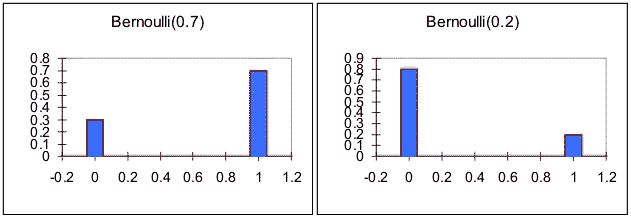
\includegraphics[scale=0.40]{bernoulli}
  \end{figure}

This picture is called the \textbf{probability mass function} of the
distribution.
\end{frame}
%

%
\begin{frame}

  \begin{figure}
    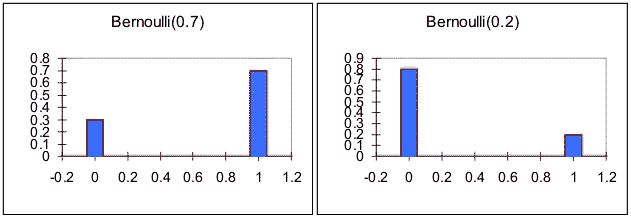
\includegraphics[scale=0.40]{bernoulli}
  \end{figure}

Notice how the first picture represents the occurrence of a \textbf{common event}
and the second a \text{rare event}.

\end{frame}
%

%
\begin{frame}

Changing the probability that the event occurs changes the shape of the
probability mass function. This is called \textbf{varying a parameter}.

  \begin{figure}
    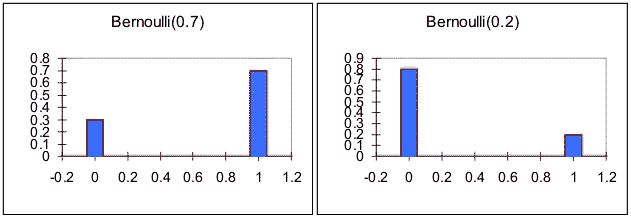
\includegraphics[scale=0.40]{bernoulli}
  \end{figure}

\end{frame}
%

%
\begin{frame}
Draw pictures of the probability mass functions of the following Bernoulli
distributions:

\begin{itemize}
\item Flipping a fair coin.
\item Rolling a six on a six sided die.
\item Rolling a twenty on a twenty sided die.
\item Rolling greater than a ten on a twenty sided die.
\end{itemize}

Are any of these equally distributed?
\end{frame}
%

%
\begin{frame}{Binomial Distribution}
The two familiar random variables

\begin{itemize}
\item The number of heads seen in ten flips of a quarter.
\item The number of heads seen in ten flips of a dime.
\end{itemize}

Have a \textbf{binomial distribution}.
\end{frame}
%

%
\begin{frame}

\begin{align*}
P(\text{We get} & \text{ 2 heads in 10 flips of a quarter}) \\
%
&= {{10}\choose{2}} \times \left(\frac{1}{2} \right)^{10} \\
%
&= 0.044
\end{align*}

\end{frame}
%

%
\begin{frame}

The \textbf{binomial distribution} describes the number of events that happen in
a fixed number of \textbf{attempts} when the events \textbf{individually happen
with the same probability}.

\end{frame}
%

%
\begin{frame}
When we are flipping a fair coin, the heads happen with probability $\frac{1}{2}$, and

\begin{align*}
P(\text{We get} & \text{ k heads in n flips of a coin}) \\
%
&= {{n}\choose{k}} \times \left(\frac{1}{2} \right)^n
\end{align*}

\end{frame}
%

%
\begin{frame}
If the coin in \textbf{unfair}, so that the probability of an individual head is
$p$, then

\begin{align*}
P(\text{We get} & \text{ k heads in n flips of an unfair coin}) \\
%
&= {{n}\choose{k}} \times p^k \times (1 - p)^{n - k}
\end{align*}

\end{frame}
%

%
\begin{frame}
The binomial distribution has \textbf{two parameters}:

\begin{itemize}
\item The number of attempts, usually called $n$.
\item The probability the event occurs in a single attempt, usually called $p$.
\end{itemize}

\end{frame}
%

%
\begin{frame}
Changing either $n$ or $p$ changes the shape of the binomial probability mass
function.

  \begin{figure}
    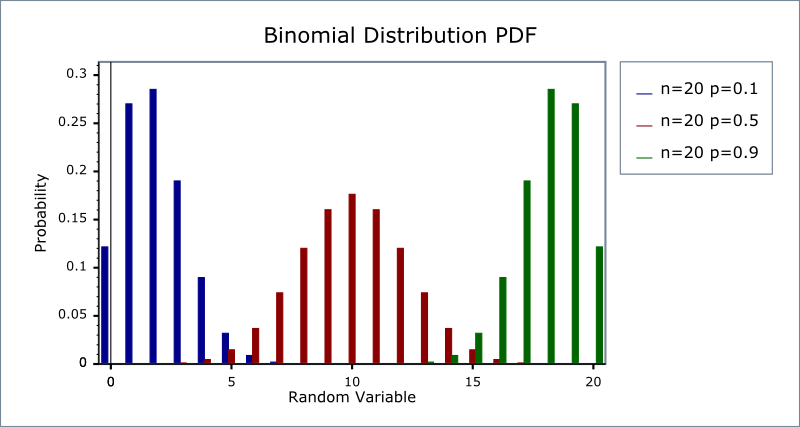
\includegraphics[scale=0.50]{binomial-pdf-changing-p}
  \end{figure}

\end{frame}
%

%
\begin{frame}

  \begin{figure}
    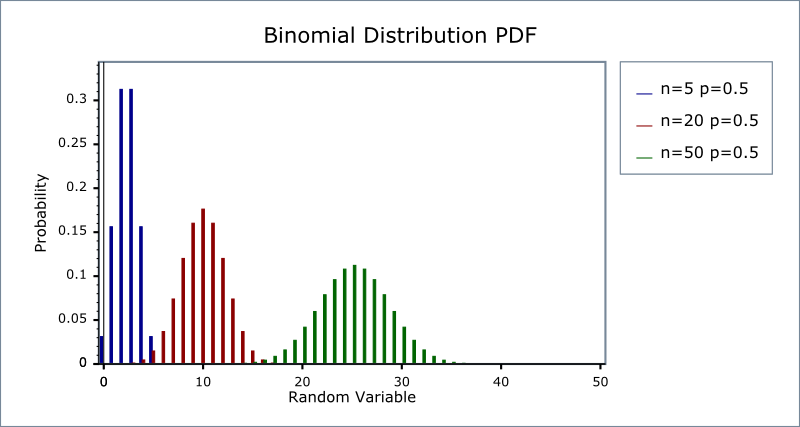
\includegraphics[scale=0.5]{binomial-pdf-changing-n}
  \end{figure}

\end{frame}
%

%
\begin{frame}

A \text{critical hit} is a roll of 20 on a 20 sided die.  In a session of
Dungeons and Dragons, you roll the die 20 times.  What is the probability that
you roll \textbf{at least two} critical hits.

\hfill

A \text{saving throw} is a roll of at least 15 on a 20 sided die.  In a session
of Dungeons and Dragons you roll the die to attempt a saving throw 10 times.
What is the probability you \text{fail} all of your saving throws?

\end{frame}
%

%
\begin{frame}{Poisson Distribution}

\begin{itemize}
\item The number of buses that arrive late to a stop in Seattle in a single
day.
\item The number of times my cat asks for food between 5 and 6 pm (when she is
always fed) in a given day.
\end{itemize}

We see a similarity: they are both about the number of times an event happens
\textbf{in a given span of time (or space)}.
\end{frame}
%

%
\begin{frame}
If we assume that the buses arrive at a fixed rate (but possibly unknown), and
the cat meows at a fixed rate, then these are both examples of the
\textbf{Poisson Distribution}.

$$ P(\text{Cat meows k times in one hour}) = e^{-\lambda} \frac{\lambda^k}{k!}
$$

The $\lambda$ above is the \textbf{rate the event occurs}.
\end{frame}
%

%
\begin{frame}
Suppose we observe the cat meow 5 times in ten minutes.  What is the probability
that the cat will not meow at all in the next ten minutes?
\end{frame}
%

%
\begin{frame}
The rate the cat meows is:

$$ \lambda = \frac{5 \text{ meows}}{10 \text{ minuets}} = 5 \frac{ \text{
meows}}{\text{ 10 minuets}} $$

So using the Poisson equation

$$ P(\text{Cat meows zero times in ten minuets}) = e^{-5} \frac{5^0}{0!} = 0.007
$$
\end{frame}
%

%
\begin{frame}
What is the probability the cat meows zero times in the next hour?

$$ 
\lambda = \frac{5 \text{ meows}}{10 \text{ minuets}} = 30 \frac{ \text{
meows}}{\text{ 60 minuets}} = 30 \frac{ \text{
meows}}{\text{ hour}}
$$

$$ P(\text{Cat meows zero times in the next hour}) = e^{-30} \frac{5^0}{0!} =
9.3 \times 10^{-14}
$$

...it's basically impossible.
\end{frame}
%

%
\begin{frame}

In the same cat problem setup, what is the probability the cat meows at
least two times in the next ten minuets?

\hfill

In a batch of cookie batter, you dump in 100 chocolate chips and then mix the
result thoroughly.  You then portion out 20 equally sized cookies.  What is the
probability that at least one cookie has no chocolate chips in it?

\end{frame}
%

%
\begin{frame}{Overview}
The general strategy for solving problems using probability distributions like is:

\begin{itemize}
\item Use the information in the statement of the problem to determine a likely
distribution for the quantity of interest.
\item Use the information in the problem to determine the values to use for the
parameters of this distribution.
\item Use the probability function of the distribution to compute the needed
probability.
\end{itemize}

You may have to break the problem down into multiple steps to succeed.  Practice
and you'll start to see common patterns!

\end{frame}
%

%
\begin{frame}

The distributions we discussed are \textbf{discrete}: the outcomes can only be
individualized numbers (0, 1, 2, 3, ...).  

\hfill

There are also \textbf{continuous distributions}.


\end{frame}
%

%
\begin{frame}{Normal Distribution}
This distribution usually shows up due to the \textbf{central limit theorem}.

\hfill

\textbf{Parameters:} The mean $\mu$, and the standard deviation $\sigma$.

  \begin{figure}
    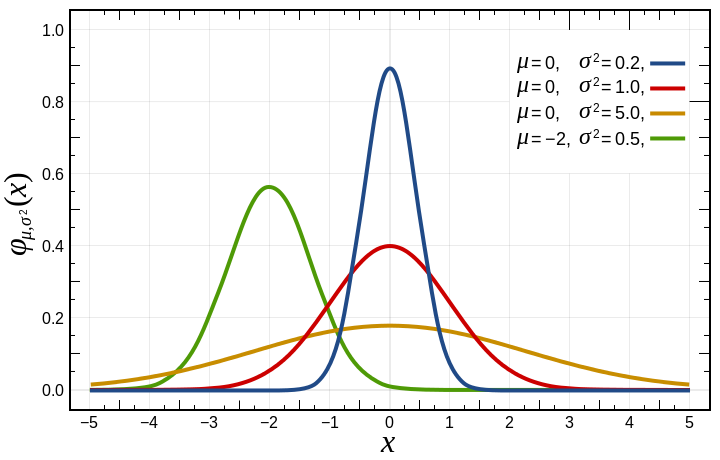
\includegraphics[scale=0.25]{normal-pdf}
  \end{figure}

\end{frame}
%

%
\begin{frame}{Uniform Distribution}
This distribution shows up when when a random event can take any value in a
range, each result being equally likely.

\hfill

\textbf{Parameters:} The minimum $a$ and the maximum $b$.

  \begin{figure}
    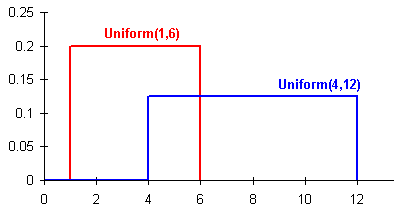
\includegraphics[scale=0.5]{uniform-pdf}
  \end{figure}

\end{frame}
%

%
\begin{frame}{Exponential Distribution}
This distribution describes the \textbf{time you have to wait before observing
an event} when the events happen at a fixed rate.

\hfill

\textbf{Parameters:} The rate $\alpha$.

  \begin{figure}
    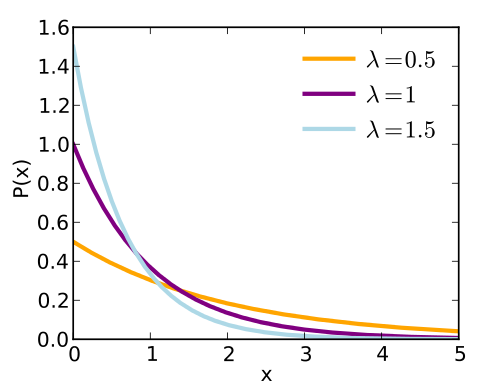
\includegraphics[scale=0.4]{exponential-pdf}
  \end{figure}

\end{frame}
%
